\documentclass[14pt]{extarticle}
\usepackage{fontspec}
\usepackage{polyglossia}
\usepackage{amsmath}
\usepackage{amssymb}
\usepackage{xcolor}
\usepackage{fancyhdr}
\usepackage{graphicx}
\usepackage{listings}
\usepackage[most]{tcolorbox}
% \usepackage{setspace}
\usepackage{pifont}
\usepackage{enumitem}
\usepackage{titlesec}
\usepackage[bottom]{footmisc}
\usepackage{titling}
\usepackage{minted}
\usepackage{etoolbox}
\usepackage{array}
\usepackage{extsizes}
\usepackage{float}
\usepackage{booktabs}
\usepackage{hyperref}
\usepackage[onehalfspacing]{setspace}
\newif\ifcolorblind
\ifdefined\setcolorblind
  \setcolorblind
\fi

\ifcolorblind
  \usepackage[a4paper, landscape, top=1cm, bottom=1cm, left=1cm, right=1cm, headheight=1.5cm, headsep=0.5cm]{geometry}
\else
  \usepackage[a4paper, top=2.7cm, bottom=2.7cm, left=2.5cm, right=2.5cm, headheight=1.5cm, headsep=0.5cm]{geometry}
\fi
\usepackage{tikz}
\usepackage{datetime2}

\usetikzlibrary{automata, positioning, arrows.meta, arrows}

\newfontfamily\emoji{Segoe UI Emoji}

\pagestyle{fancy}

\setmainlanguage[numerals=western]{arabic}
\setotherlanguage{english}
\newfontfamily\arabicfont[Script=Arabic]{Calibri}
\newfontfamily\arabicfonttt[Script=Arabic]{Courier New}



\ifcolorblind
\lstset{
  language=[Sharp]C,
  numbers=left,
  stepnumber=1,
  numbersep=8pt,
  frame=single,
  basicstyle=\ttfamily\small,
  keywordstyle=\bfseries,
  stringstyle=\ttfamily,
  commentstyle=\itshape
}
\else
\lstset{
  language=[Sharp]C,
  numbers=left,
  stepnumber=1,
  numbersep=8pt,
  frame=single,
  basicstyle=\ttfamily\small,
  keywordstyle=\color{blue},
  stringstyle=\color{red},
  commentstyle=\color{green!50!black}
}
\fi

\newif\ifdetailed
\ifdefined\setdetailed
  \setdetailed
\fi

\newif\ifwithsols
\ifdefined\setwithsols
  \setwithsols
\fi

\ifcolorblind
  \AtBeginDocument{
    \LARGE
    \usemintedstyle{bw}
  }
\fi

% unified tcolorboxes for articles
\ifcolorblind
\tcbset{colback=white, colframe=black, fonttitle=\bfseries, boxrule=1pt}
\newtcolorbox{boxDef}[1][]{title={{\emoji📘} تعريف\ifx\\#1\\\else ~#1\fi :}}
\newtcolorbox{boxExercise}[1][]{title={{\emoji🧩} تمرين\ifx\\#1\\\else ~#1\fi :}}
\newtcolorbox{boxExample}[1][]{title={{\emoji📝} مثال\ifx\\#1\\\else ~#1\fi :}}
\newtcolorbox{boxNote}[1][]{title={{\emoji✨} ملاحظة\ifx\\#1\\\else ~#1\fi :}}
\newtcolorbox{boxAttention}[1][]{title={{\emoji🔔} تنبيه\ifx\\#1\\\else ~#1\fi :}}
\newtcolorbox{boxWarning}[1][]{title={{\emoji⚡} ملاحظة هامة\ifx\\#1\\\else ~#1\fi :}}
\newtcolorbox{boxSolution}[1][]{title={{\emoji✅} حل\ifx\\#1\\\else ~#1\fi :}}
\newtcolorbox{boxSymbol}[1][]{title={{\emoji🔣} رمز\ifx\\#1\\\else ~#1\fi :}}
\newtcolorbox{boxHint}[1][]{title={{\emoji💡} تلميح\ifx\\#1\\\else ~#1\fi :}}
\else
\tcbset{colback=white, colframe=black, fonttitle=\bfseries, boxrule=0.8pt}
\newtcolorbox{boxDef}[1][]{colback=blue!5!white,colframe=blue!75!black,
  title={{\emoji📘} تعريف\ifx\\#1\\\else ~#1\fi :}}
\newtcolorbox{boxExercise}[1][]{colback=cyan!5!white,colframe=cyan!70!black,
  title={{\emoji🧩} تمرين\ifx\\#1\\\else ~#1\fi :}}
\newtcolorbox{boxExample}[1][]{colback=yellow!5!white,colframe=orange!90!black,
  title={{\emoji📝} مثال\ifx\\#1\\\else ~#1\fi :}}
\newtcolorbox{boxNote}[1][]{colback=gray!10!white,colframe=black,
  title={{\emoji✨} ملاحظة\ifx\\#1\\\else ~#1\fi :}}
\newtcolorbox{boxAttention}[1][]{colback=magenta!10!white,colframe=magenta!80!black,
  title={{\emoji🔔} تنبيه\ifx\\#1\\\else ~#1\fi :}}
\newtcolorbox{boxWarning}[1][]{colback=red!5!white,colframe=red!75!black,
  title={{\emoji⚡} ملاحظة هامة\ifx\\#1\\\else ~#1\fi :}}
\newtcolorbox{boxSolution}[1][]{colback=green!5!white,colframe=green!60!black,
  title={{\emoji✅} حل\ifx\\#1\\\else ~#1\fi :}}
\newtcolorbox{boxSymbol}[1][]{colback=purple!5!white,colframe=purple!70!black,
  title={{\emoji🔣} رمز\ifx\\#1\\\else ~#1\fi :}}
\newtcolorbox{boxHint}[1][]{colback=teal!5!white,colframe=teal!60!black,
  title={{\emoji💡} تلميح\ifx\\#1\\\else ~#1\fi :}}
\fi


\ifcolorblind
\tcbset{simplecode/.style={ colback=white, colframe=black, boxrule=1pt, arc=2pt, left=4pt,right=4pt,top=4pt,bottom=4pt}}
\else
\tcbset{simplecode/.style={ colback=gray!5, colframe=black!50, boxrule=0.4pt, arc=2pt, left=4pt,right=4pt,top=4pt,bottom=4pt}}
\fi
\newenvironment{boxCode}{\begin{tcolorbox}[simplecode]}{\end{tcolorbox}}

\newcolumntype{C}[1]{>{\centering\arraybackslash}p{#1}}

\makeatletter
\DTMnewdatestyle{dotted}{%
  \renewcommand{\DTMdisplaydate}[4]{\two@digits{##3}.\two@digits{##2}.##1}%
  \renewcommand{\DTMDisplaydate}{\DTMdisplaydate}%
}
\makeatother
\DTMsetdatestyle{dotted}

% redefine spaces after titles
\makeatletter
\renewcommand{\@maketitle}{%
  \begin{center}
    {\huge \bfseries \@title \par}%
    \vskip 0.2em % space between title and author
    {\large \@author \par}%
    % \vskip 0.2em % space between author and date
    % {\normalsize \@date \par}%
    {\small \hfill \begin{english}\DTMtoday\end{english} \par}%
  \end{center}
}
\makeatother

\fancyhf{} % clear default
\fancypagestyle{plain}{
  \fancyhf{}
  \fancyhead[L]{مدرسة التسامح الشاملة}
  % \fancyhead[L]{
\includegraphics[height=1cm]{../../../images/logoTasamoh.png}}
  \fancyhead[R]{الأستاذ محمود اغبارية}
  \fancyfoot[C]{\thepage}
}

\fancyhead[L]{مدرسة التسامح الشاملة}
\fancyhead[R]{الأستاذ محمود اغبارية}
\fancyfoot[C]{\thepage}

\setcounter{tocdepth}{3} % only section subsection and subsubsection in TOC

\newcommand{\importpdfpage}[2]{%
    \thispagestyle{empty}
    \newgeometry{left=0cm,right=0cm,top=0cm,bottom=0cm}
    \includegraphics[page=#2,width=0.95\paperwidth,height=0.95\paperheight,keepaspectratio]{#1}
    \restoregeometry
}

\newcommand{\insertFullImg}[1]{%
    \noindent
    \makebox[\textwidth][c]{
        \includegraphics[width=0.9\paperwidth,keepaspectratio]{#1}%
    }%
}%

% ----------------------


% \begin{document}

% \maketitle

% % \clearpage  % start TOC on a new page
% % \renewcommand{\contentsname}{جدول المحتويات}
% % \tableofcontents
% % \clearpage

% \part*{part 1} % the * prevents numbering
% \section*{مقدمة}
% \subsection*{مثال رياضي}
% \subsubsection*{مثال فرعي}
% \paragraph*{ paragraph 1}
% \subparagraph*{sub paragraph 1}

% \ifdetailed
% \begin{english}
% \begin{minted}{csharp}
% // C# Example
% \end{minted}
% \end{english}
% \fi

% OLD WAY
% \ifdetailed
% \begin{english}
% \begin{lstlisting}
% // C# Example
% \end{lstlisting}
% \end{english}
% \fi

% % 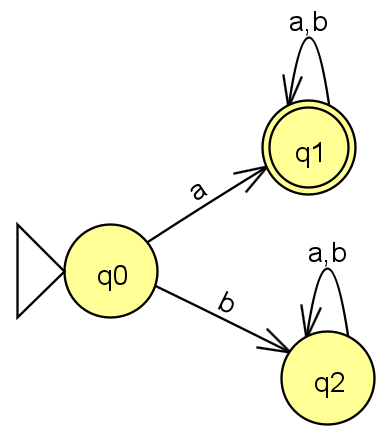
\includegraphics[width=0.2\textwidth]{../../../images/DFAs/ex1_q1.png}



% \vspace{3cm}
% \begin{flushleft}
% أرجو لكم وقتًا ممتعًا.

% الأستاذ محمود اغبارية.
% \end{flushleft}


% \end{document}


\title{ورقة تمرن 4: المتغيرات ومكتبة \textenglish{Math}}

\begin{document}

\maketitle
\thispagestyle{fancy}

\begin{enumerate}[itemsep=3em]

    \item
    اكتب برنامجًا يستقبل من المستخدم عددًا من 3 منازل (مثلاً 258)، ويقوم ببناء عدد جديد بحيث تكون منازله معكوسة (852). ثم يطبع العدد الجديد، ويحسب ويطبع الفارق المطلق بين العدد الأصلي والعدد المعكوس.
    \ifdetailed
    \begin{boxExample}
    \begin{english}
    \begin{minted}{csharp}
Please enter a 3-digit number:
258
Reversed number = 852
Absolute difference = 594
    \end{minted}
    \end{english}
    \end{boxExample}
    \ifwithsols
    \begin{boxSolution}
    \begin{english}
    \begin{minted}{csharp}
int num = int.Parse(Console.ReadLine());
int units = num % 10;
num = num / 10;
int tens = num  % 10;
int hundreds = num / 100;

int reversedNum = units * 100 + tens * 10 + hundreds;
int diff = Math.Abs(num - reversedNum);

Console.WriteLine("Reversed number = " + reversedNum);
Console.WriteLine("Absolute difference = " + diff);
    \end{minted}
    \end{english}
    \end{boxSolution}
    \clearpage
    \fi
    \fi

    \ifwhiteblack
    \clearpage
    \fi

    \item
    اكتب برنامجًا يستقبل من المستخدم عددًا يمثل مبلغًا من المال (من مضاعفات الـ $50$)، ويطبع أقل عدد ممكن من الأوراق النقدية (فئة 200، 100، 50) اللازمة لتكوين هذا المبلغ.
    \ifdetailed
    \begin{boxExample}
    \begin{english}
    \begin{minted}{csharp}
Please enter the amount:
878
200 bills: 4
100 bills: 0
50 bills: 1
    \end{minted}
    \end{english}
    \end{boxExample}
    \ifwithsols
    \begin{boxSolution}
    \begin{english}
    \begin{minted}{csharp}
int amount = int.Parse(Console.ReadLine());

int bills200 = amount / 200;
amount = amount % 200;

int bills100 = amount / 100;
amount = amount % 100;

int bills50 = amount / 50;
amount = amount % 50;

Console.WriteLine("200 bills: " + bills200);
Console.WriteLine("100 bills: " + bills100);
Console.WriteLine("50 bills: " + bills50);
    \end{minted}
    \end{english}
    \end{boxSolution}
    \fi
    \fi
    \clearpage

    \item
    اكتب برنامجًا يستقبل وقتين (وقت بداية حدث ووقت نهايته) كأعداد صحيحة من 4 منازل بنظام 24 ساعة (مثلاً 1430 تعني 14:30).
    البرنامج يحسب مدة الحدث بالدقائق الإجمالية ويطبعها.
    \ifdetailed
    \begin{boxExample}
    \begin{english}
    \begin{minted}{csharp}
Please enter start time (HHMM):
1430
Please enter end time (HHMM):
1615
Duration in minutes = 105
    \end{minted}
    \end{english}
    \end{boxExample}
    \ifwithsols
    \begin{boxSolution}
    \begin{english}
    \begin{minted}{csharp}
int start = int.Parse(Console.ReadLine());
int end = int.Parse(Console.ReadLine());

int startHours = start / 100;
int startMinutes = start % 100;
int startTotalMins = startHours * 60 + startMinutes;

int endHours = end / 100;
int endMinutes = end % 100;
int endTotalMins = endHours * 60 + endMinutes;

int duration = endTotalMins - startTotalMins;
Console.WriteLine("Duration in minutes = " + duration);
    \end{minted}
    \end{english}
    \end{boxSolution}
    \clearpage
    \fi
    \fi
    \ifwhiteblack
    \clearpage
    \fi

    \item
    اكتب برنامجًا يستقبل محيط مربع.
    البرنامج يقوم بحساب وطباعة مساحة هذا المربع.
    ثم، بافتراض وجود دائرة لها \textbf{نفس مساحة هذا المربع}، البرنامج يقوم بحساب نصف قطر هذه الدائرة وتقريبه لمنزلتين عشريتين باستخدام الدالة $\mathtt{Math.Round}$، ومن ثم يطبعه. \\
    ($\text{المساحة} = 3.14 \times r^2 \Rightarrow r = \sqrt{\frac{\text{المساحة}}{3.14}}$)
    \ifdetailed
    \begin{boxExample}
    \begin{english}
    \begin{minted}{csharp}
Please enter the square's perimeter:
20
Square Area = 25
Circle Radius (rounded) = 2.82
    \end{minted}
    \end{english}
    \end{boxExample}
    \ifwithsols
    \begin{boxSolution}
    \begin{english}
    \begin{minted}{csharp}
double perimeter = double.Parse(Console.ReadLine());

double side = perimeter / 4.0;
double squareArea = Math.Pow(side, 2);
Console.WriteLine("Square Area = " + squareArea);

double radiusSq = squareArea / 3.14;
double radius = Math.Sqrt(radiusSq);

double rTimes100 = radius * 100;
double rRounded = Math.Round(rTimes100);
double finalRadius = rRounded / 100.0;

Console.WriteLine("Circle Radius (rounded) = " + finalRadius);
    \end{minted}
    \end{english}
    \end{boxSolution}
    \fi
    \fi
    \clearpage

    \item
    اكتب برنامجًا يستقبل من المستخدم عددًا عشريًّا يمثّل قيمة $x$.
    البرنامج يقوم بحساب وطباعة قيمة الدالة التالية عند النقطة $x$:
    $$ f(x) = \frac{x + 1}{x^3} $$
    (افترض أن المدخلات دائما صحيحة ولا تسبب خطأ رياضي).
    \ifdetailed
    \begin{boxExample}
    \begin{english}
    \begin{minted}{csharp}
Please enter x:
2
f(x) = 0.375
    \end{minted}
    \end{english}
    \end{boxExample}
    \ifwithsols
    \begin{boxSolution}
    \begin{english}
    \begin{minted}{csharp}
double x = double.Parse(Console.ReadLine());

double num = x + 1;
double den = Math.Pow(x, 3);
double result = num / den;

Console.WriteLine("f(x) = " + result);
    \end{minted}
    \end{english}
    \end{boxSolution}
    \clearpage
    \fi
    \fi
    \ifwhiteblack
    \clearpage
    \fi

    \item
    اكتب برنامجًا يستقبل من المستخدم عددًا عشريًّا يمثّل قيمة $x$.
    البرنامج يقوم بحساب وطباعة قيمة الدالة التالية عند النقطة $x$:
    $$ f(x) = (\sqrt{x} + 1)^2 $$
    (افترض أن المدخلات دائما صحيحة ولا تسبب خطأ رياضي).
    \ifdetailed
    \begin{boxExample}
    \begin{english}
    \begin{minted}{csharp}
Please enter x:
4
f(x) = 9
    \end{minted}
    \end{english}
    \end{boxExample}
    \ifwithsols
    \begin{boxSolution}
    \begin{english}
    \begin{minted}{csharp}
double x = double.Parse(Console.ReadLine());

double root = Math.Sqrt(x);
double inner = root + 1;
double result = Math.Pow(inner, 2);

Console.WriteLine("f(x) = " + result);
    \end{minted}
    \end{english}
    \end{boxSolution}
    \fi
    \fi

    \clearpage
    \item
    اكتب برنامجًا يستقبل من المستخدم عددًا عشريًّا يمثّل قيمة $x$.
    البرنامج يقوم بحساب وطباعة قيمة الدالة التالية عند النقطة $x$:
    $$ f(x) = \frac{|x^3 - 8|}{\sqrt{x^2 + 16}} $$
    (افترض أن المدخلات دائما صحيحة ولا تسبب خطأ رياضي).
    \ifdetailed
    \begin{boxExample}
    \begin{english}
    \begin{minted}{csharp}
Please enter x:
3
f(x) = 3.8
    \end{minted}
    \end{english}
    \end{boxExample}
    \ifwithsols
    \begin{boxSolution}
    \begin{english}
    \begin{minted}{csharp}
double x = double.Parse(Console.ReadLine());

double num = Math.Abs(Math.Pow(x, 3) - 8);
double den = Math.Sqrt(Math.Pow(x, 2) + 16);
double result = num / den;

Console.WriteLine("f(x) = " + result);
    \end{minted}
    \end{english}
    \end{boxSolution}
    \fi
    \fi

\end{enumerate}

\end{document}
